\chapter{Towards Reliable Systems of Twinned Systems}\label{ch:approach}
This chapter presents an approach to building reliability in SoTS. Building on the gaps identified in the literature review, it formalizes reliability in the context of constituent lifecycle dynamics and defines explicit levels of reliability under disturbance and reconfiguration. The chapter establishes a structured foundation for modeling, assessing, and preserving SoTS operation.

\section{Reliability in SoTS}
Reliability, in classical dependability theory, is defined as the probability that a system performs its intended function without failure for a specified period of time \cite{avizienis2004basic}. In SoS, this notion must be extended to account for operational independence, dynamic reconfiguration, and emergent behavior among constituent systems. Accordingly, reliability is increasingly reframed in terms of disturbances rather than isolated component faults \cite{ferreira2023towards}. 
Disturbances may arise from constituent failures, communication breakdowns, organizational factors, or independent evolution that misaligns services \cite{ferreira2021reliability}.
Because constituents are interdependent, such disturbances propagate across system boundaries and impact mission fulfillment. Reliability in SoS therefore concerns sustaining system-level capabilities despite ongoing disturbance, evolution, and reconfiguration.



% These challenges are amplified in SoTS.
These disturbance dynamics are amplified in SoTS. DTs depend on continuous and timely information exchange between physical and digital constituents. In an evolving SoS environment, observation availability, timing guarantees, and participation cannot be assumed stable. Delayed or incomplete information introduces uncertainty into the digital layer and may compromise coordinated behavior. In SoTS, reliability therefore depends on maintaining acceptable system operation despite fluctuating participation and imperfect information.
% In SoTS, reliability ultimately concerns sustaining system capabilities even as constituent availability and information quality vary over time.

The systematic literature review (\secref{sec:literature-review-key-takeaways}) confirms this gap. Although reliability is frequently cited as a motivation or quality attribute in SoTS studies, it is rarely modeled explicitly or validated at runtime. Most contributions address reliability indirectly through structural redundancy, communication fallback mechanisms, state persistence, or distributed deployment architectures, rather than treating it as an operational property that must be formally assessed and maintained during execution.



\begin{table*}[t]
\small
\centering
\caption{SoS Reliability Strategies with \citet{hanmer2013patterns} Fault-Tolerance Pattern Families}
\label{tab:sos-reliability-techniques}
\renewcommand{\arraystretch}{1.25}
\begin{tabular}{p{3.5cm} p{3.5cm} p{7.5cm}}
\toprule
\textbf{Pattern Family} & \textbf{SoS Reliability Strategy} & \textbf{Techniques Identified \cite{ferreira2021reliability, uday2015designing, abdelmoumen2026comprehensive}} \\
\midrule

\textbf{Architectural Patterns} 
& Structural Redundancy and Substitution 
& Spatial redundancy; functional redundancy; constituent replication; Substitutable Heterogeneous System Architectures (SHSA) \\


\midrule

\textbf{Error Detection} 
& Runtime Monitoring and Verification 
& Fault Detection and Isolation (FDI); runtime verification using Linear Temporal Logic (LTL) and Computation Tree Logic (CTL); anomaly detection \\

\midrule

\textbf{Error Recovery} 
& Task and Goal Reallocation 
& Multi-objective optimization (e.g., NSGA-II) for task redistribution and mission re-planning; dynamic task reassignment; architectural reconfiguration \\


\midrule

\textbf{Error Mitigation} 
& Estimation and Prediction 
& Kalman filtering; Neural Network  prediction (e.g., Long Short-Term Memory (LSTM)); Time-series forecasting\\

\midrule

\textbf{Fault Treatment} 
& Dependency, Probabilistic, and Hazard Modeling 
& Functional Dependency Network Analysis (FDNA); Bayesian Networks; Markov chains and Continuous-Time Markov Models (CTMM); Petri nets; Monte Carlo simulation; 
\newline
Failure Mode and Effects Analysis (FMEA); Failure Mode, Effects, and Criticality Analysis (FMECA); Fault Tree Analysis (FTA); Event Tree Analysis (ETA); Hazard and Operability Study (HAZOP) \\

\bottomrule
\end{tabular}
\end{table*}

\section{Existing Strategies for Reliable SoTS}
Techniques for preserving reliability in SoS align closely with the fault-tolerance pattern families described by \citet{hanmer2013patterns}. As summarized in \tabref{tab:sos-reliability-techniques}, the approaches identified in major SoS reliability surveys \cite{ferreira2021reliability, uday2015designing, abdelmoumen2026comprehensive} span: architectural mechanisms (structural organization and redundancy to contain faults), error detection (mechanisms to identify abnormal behavior at runtime), error recovery (strategies to restore acceptable operation after disruption), error mitigation (techniques that limit the impact of errors during operation), and fault treatment (analysis and modeling approaches that identify, diagnose, or eliminate underlying causes).

Existing SoTS studies predominantly emphasize architectural patterns and error mitigation mechanisms. Most implementations rely on structural redundancy and component substitution, including fallback communication layers, state persistence, distributed or cloud-based DT deployment, asynchronous messaging, and data caching during disconnection \cite{acharya2023twins, aziz2022empowering, larsen2024towards, lopez2023modeling}. Error detection is occasionally supported through runtime monitoring, event-triggered replanning, or dynamic rescheduling \cite{park2020digital, villalonga2021decision-making}. In contrast, comparatively few studies incorporate explicit fault treatment approaches such as parametric reliability modeling, uncertainty reasoning, or fault tree analysis (FTA) \cite{kutzke2021subsystem, oquendo2019dealing, saraeian2022digital}. 


\section{Ensuring Reliable Participation and Stable Operation in SoTS}
A foundational principle in SoS architecting is the notion of \emph{stable intermediate forms} \cite{maier1998architecting}: partial configurations must remain operational and capable of delivering useful functionality throughout deployment, evolution, and reconfiguration. Subsequent work reinforces this view, arguing that SoS evolution must proceed through viable configurations that preserve value and maintain service continuity during adaptation \cite{rechtin1991systems, rechtin2010art, mekdeci2014pliability, petitdemange2021design, weyns2013challenges}. 

In practice, however, maintaining such stable intermediate forms is difficult because SoS configurations are not static. Reconfiguration is intrinsic to SoS evolution: constituents may join, leave, degrade, suspend participation, or shift roles over time \cite{fang2020improving, manzano2020dynamic, pradhan2016achieving, mohsin2019modeling}. As participation changes, the operational boundary of the SoTS shifts, introducing structural reconfiguration and uncertainty about constituent state and availability. Reliability must therefore be preserved not within a fixed architecture, but across continuously evolving compositions. Without an explicit model of membership transitions, reliability mechanisms respond to isolated disruptions rather than systematically managing how system configurations change over time.

SoS research has increasingly formalized constituent lifecycle states. \citet{axelsson2019refined} distinguish ignorant, prepared, passive, and active states; \citet{hristozov2023modeling} define a state machine governing safe initialization and withdrawal; \citet{petitdemange2021design} structure reconfiguration through coordinated active-passive transitions; and other work models negotiation states \cite{qin2016contract}, standby and replacement roles \cite{du2024reconfiguration}, or lifecycle-driven situational awareness \cite{svenson2020situation}. 

In SoTS, these transitions directly affect the availability and consistency of digital representations. To preserve stable intermediate forms, participation changes must therefore be bounded, coordinated, and, when necessary, compensated. The remainder of this section derives explicit reliability requirements from constituent lifecycle management and introduces levels of operational reliability that characterize how effectively a SoTS maintains functionality under reconfiguration and evolution. 


\section{Reliability Levels Through Constituent Lifecycle Control}

In SoTS, participation is not static. Digital twins join, suspend, resume, degrade, or withdraw over time. Each such transition alters the operational boundary of the SoTS. If these transitions are unmanaged, the SoTS becomes unrelaible. 

We therefore model operational reliability as progressively stronger control over constituent lifecycle within the SoTS. Each level introduces additional structure that constrains how participation evolves, extending previous levels with additional coordination and fault-tolerance mechanisms.


\paragraph{Level 1 — Uncoordinated Participation}
At the most basic level, a constituent exists in one of two states: \emph{Idle}, where it is not contributing capabilities to the SoTS, and \emph{Participating}, where it actively provides services within the current configuration. Transitions between these states occur directly and without coordination. Entry and exit are triggered implicitly through \texttt{join()}, \texttt{leave()}, or \texttt{crash()} events, and the SoTS has no prior awareness of membership changes.

\begin{figure}[t]
    \centering
    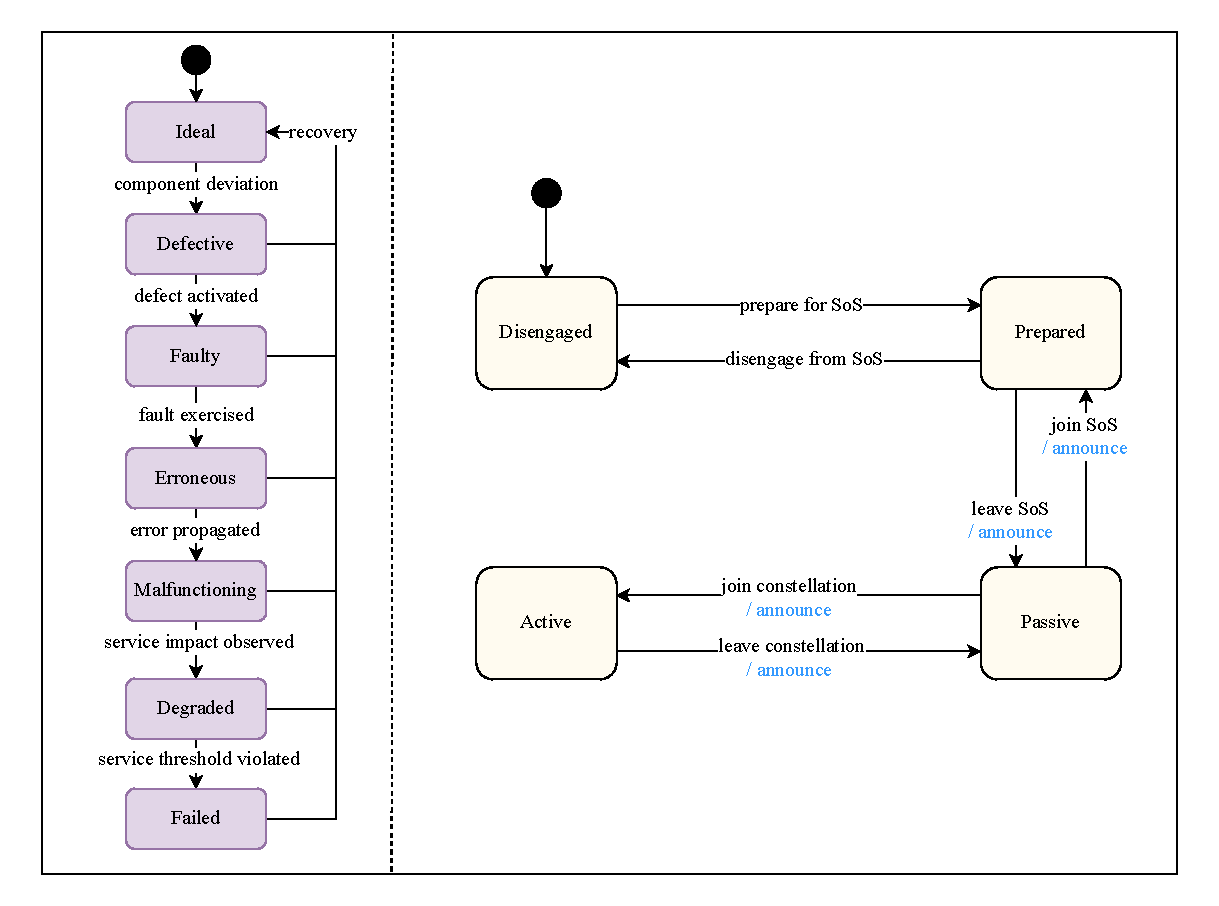
\includegraphics[width=0.6\textwidth]{figures/Approach/lv1.pdf}
    \caption{Level 1: Uncoordinated participation.}
    \label{fig:level1}
\end{figure}

Departures may therefore occur abruptly, requiring the SoTS to tolerate sudden loss of functionality. Stable intermediate forms are not explicitly enforced. Membership changes are unmanaged, and reliability mechanisms operate reactively after disruption. As a result, Level~1 provides only minimal operational reliability within the SoTS.

\paragraph{Level 2 — Announced Participation}

Level~2 introduces a third state, \emph{Standby}, which mediates transitions between \emph{Idle} and \emph{Participating}. Rather than switching states immediately, constituents announce their intent to join or leave and enter Standby for a bounded delay.

\begin{figure}[t]
    \centering
    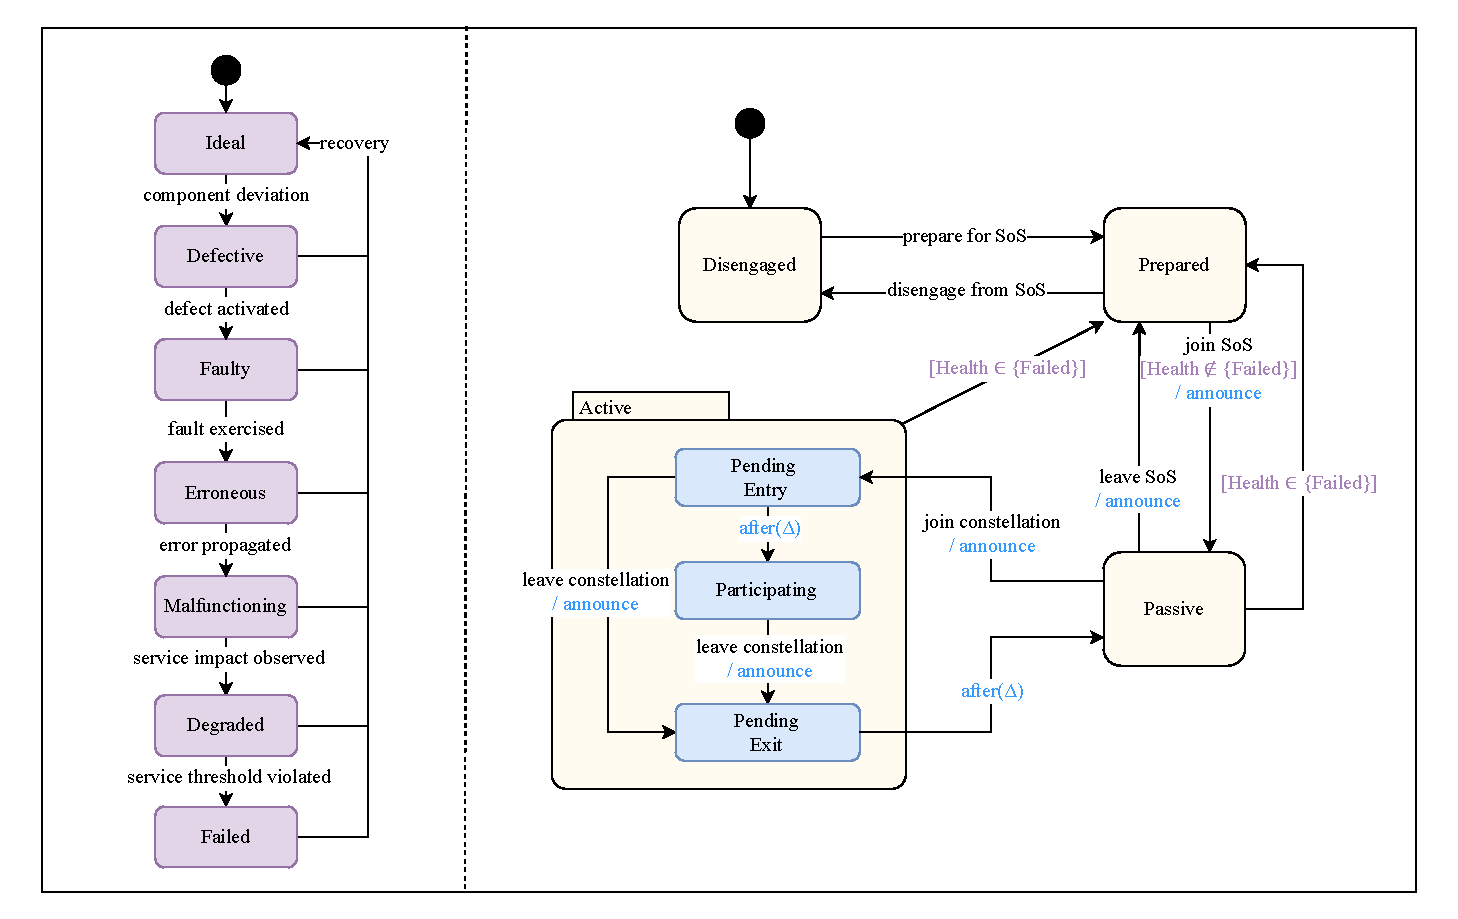
\includegraphics[width=0.6\textwidth]{figures/Approach/lv2.pdf}
    \caption{Level 2: Announced participation with bounded delay.}
    \label{fig:level2}
\end{figure}

Join and leave operations are no longer implicit. An \texttt{announceJoin()} or \texttt{announceLeave()} transition precedes activation or departure, and completion occurs only after a specified notice period (e.g., \texttt{after($t_{\text{notice}}$)}). Abrupt crashes remain possible, but voluntary transitions are now temporally bounded.

This structure improves reliability by constraining when participation changes may occur. The SoTS gains some predictability: membership evolution is no longer instantaneous, allowing time for monitoring, logging, or lightweight preparation. Level~2 therefore provides bounded but still limited operational reliability within the SoTS.


\paragraph{Level 3 — Negotiated Participation}

Level~3 introduces controlled participation through explicit negotiation. In addition to \emph{Idle}, \emph{Standby}, and \emph{Participating}, a \emph{Negotiating} state governs both entry and exit. Constituents cannot autonomously activate or withdraw. Instead, they must initiate \texttt{negotiateParticipation()} and obtain approval before transitioning.

\begin{figure}[t]
    \centering
    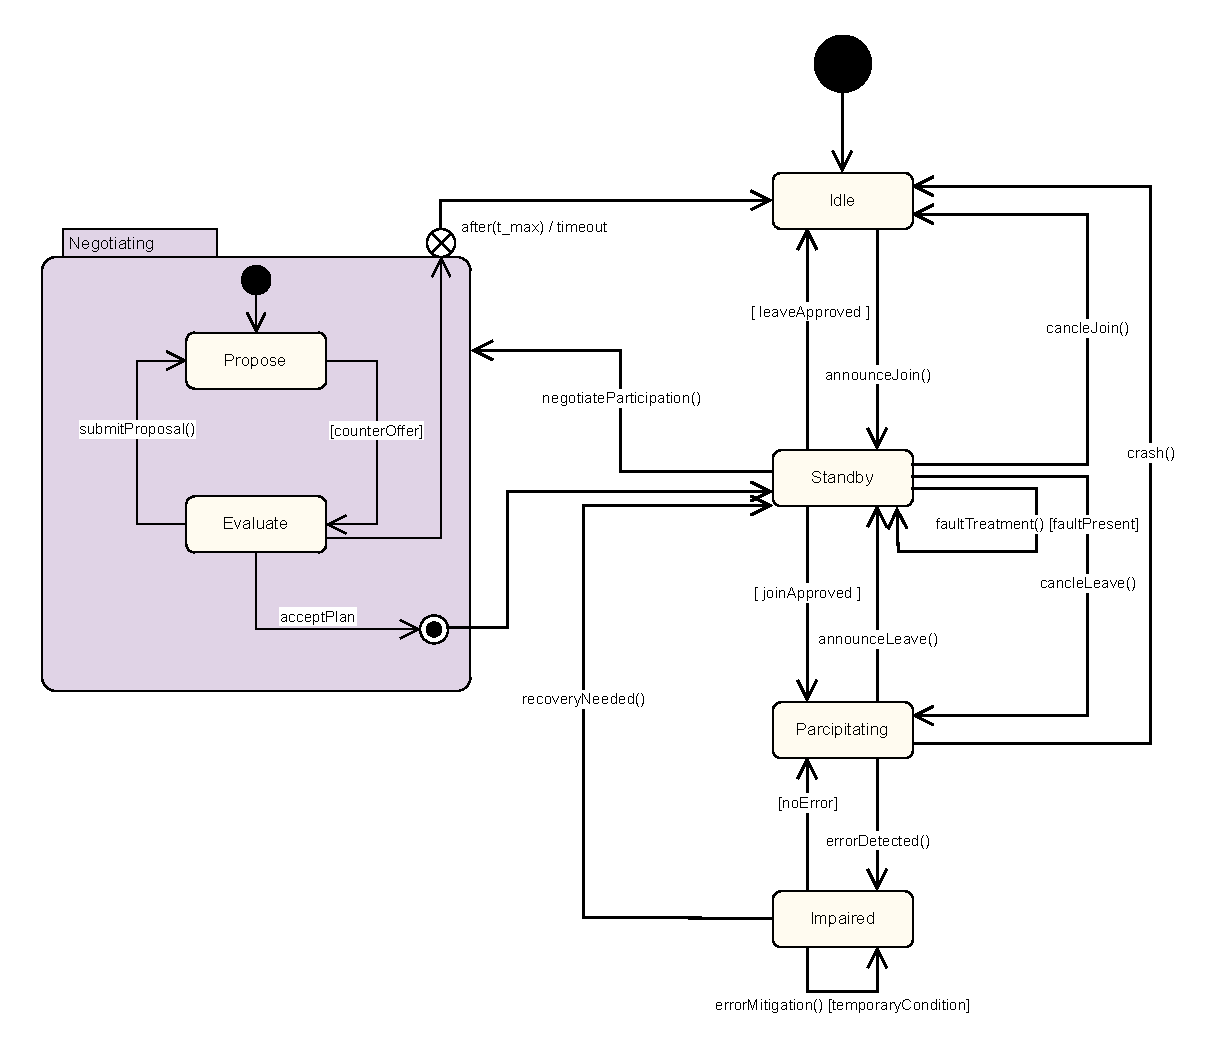
\includegraphics[width=0.6\textwidth]{figures/Approach/lv3.pdf}
    \caption{Level 3: Negotiated participation with bounded negotiation.}
    \label{fig:level3}
\end{figure}

Negotiation consists of proposal and evaluation steps (e.g., \texttt{submitProposal()}), potentially iterating under counter-offers and bounded by a maximum duration (e.g., \texttt{after($t_{\text{max}}$)}). Upon approval, the constituent returns to \emph{Standby}, from which guarded transitions (\texttt{[joinApproved]} or \texttt{[leaveApproved]}) determine activation or withdrawal. Crashes remain possible at any stage.

At this level, participation is no longer time-bounded but decision controlled. Constituents cannot independently alter the configuration; activation and withdrawal require explicit approval. Configuration evolution is therefore constrained by explicit approval logic, reducing uncoordinated reconfiguration and improving preservation of stable intermediate forms.



\paragraph{Level 4 — Fault-Aware Lifecycle with Integrated Compensation}

Level~4 embeds \citet{hanmer2013patterns} fault-tolerance pattern families directly into the constituent lifecycle. In addition to negotiated participation, constituents perform continuous \emph{error detection} through runtime monitoring. When a disturbance is detected, the lifecycle transitions from \emph{Participating} to an \emph{Impaired} state, where \emph{error mitigation} techniques may be applied to preserve temporary functionality.

If mitigation alone is insufficient, \emph{error recovery} is explicitly planned and negotiated. As shown in Figure~\ref{fig:level4}, negotiation may produce a compensation plan executed through \emph{architectural mechanisms} (e.g., redundancy activation, interface rebinding, state transfer) and recovery strategies (e.g., task reallocation). Compensation is therefore formally integrated into participation dynamics rather than invoked externally.

Once stability is restored (\texttt{[systemStable]}), the constituent re-enters normal participation. \emph{Fault treatment} may be performed while in \emph{Standby}, enabling root-cause analysis and correction without disrupting active operation.

\begin{figure}[t]
    \centering
    
\includegraphics[width=0.6\textwidth]{figures/approach/lv4.pdf}
    \caption{Level 4: Integrated fault-tolerant participation lifecycle.}
    \label{fig:level4}
\end{figure}

At this level, reliability is preserved across both configuration change and operational disturbance. Detection, mitigation, recovery, and treatment are explicitly coordinated with membership transitions. Stable intermediate forms are actively enforced through lifecycle-integrated fault management.



\section{Reliable SoTS Requirements}
\label{sec:reliable-sots-requirements}

The four reliability levels progressively introduce structure into constituent lifecycle management. From these levels, we derive a set of requirements for reliable SoTS. These requirements formalize the conditions under which stable intermediate forms can be preserved despite membership change and disturbance.

\subsection{Lifecycle Control Requirements}

\textbf{R1 — Explicit Participation States.}  
A constituent shall expose explicit lifecycle states that distinguish non-participation, transitional participation, and active participation (e.g., \emph{Idle}, \emph{Standby}, \emph{Participating}).  
\emph{Rationale:} Level~1 demonstrates that implicit transitions provide minimal reliability. Explicit states enable structured control of configuration evolution.

\textbf{R2 — Controlled Transition Semantics.}  
Transitions between participation states shall be governed by well-defined triggers, guards, and temporal constraints.  

\textbf{R3 — Bounded Reconfiguration.}  
Participation transitions shall not occur without bounded temporal or decision constraints (e.g., notice periods or negotiated approval).  

\subsection{Governance and Negotiation Requirements}

\textbf{R4 — Negotiated Activation and Withdrawal.}  
Constituents shall obtain explicit approval before activation or withdrawal from the SoTS configuration.  

\textbf{R5 — Bounded Negotiation.}  
Negotiation processes shall be temporally bounded to prevent indefinite suspension of configuration evolution.  

\subsection{Integrated Fault-Tolerance Requirements}

\textbf{R6 — Continuous Disturbance Detection.}  
Participating constituents shall perform runtime monitoring capable of detecting disturbances that threaten operational capability.  

\textbf{R7 — Lifecycle-Aware Mitigation.}  
Upon disturbance detection, constituents shall transition to a defined impaired mode where mitigation techniques may be applied without immediate withdrawal.  

\textbf{R8 — Negotiated Recovery and Compensation.}  
If mitigation is insufficient, recovery shall be planned and negotiated, and executed through architectural mechanisms (e.g., redundancy activation, state transfer, interface rebinding) and task reallocation strategies.  

\textbf{R9 — Deferred Fault Treatment.}  
Root-cause analysis and correction shall be performed in standby states when possible, preventing disruption of active service.  
\emph{Rationale:} Fault treatment should not destabilize stable intermediate forms.

\subsection{Operational Reliability Levels}

Together, these requirements define operational reliability as the degree to which participation evolution is structured, bounded, negotiated, and fault-aware.

\begin{itemize}
    \item Level~1 satisfies only R1 implicitly and provides minimal reliability.
    \item Level~2 satisfies R1-R3 through bounded participation.
    \item Level~3 satisfies R1-R5 through negotiated governance.
    \item Level~4 satisfies R1-R9 through lifecycle-integrated fault tolerance.
\end{itemize}

Operational reliability in SoTS is therefore not a static property of architecture alone, but a function of how membership transitions, disturbance handling, and compensation mechanisms are coordinated within the constituent lifecycle.
